

%!TEX root = ../dissertation.tex
\chapter{ORDINARY KRIGING FOR SPATIALLY INDEXED FUNCTIONAL DATA} 
\label{ch:functional kriging}

\section{Introduction} 

% (fold)
\label{sec:introduction}

Data that arise from measurements at geographic locations often exhibit similarities at small spatial scales. Often a primary objective of the analysis is the prediction at unobserved locations. In this setting, geostatistical models are particularly useful because the spatial process is modeled as a continuous stochastic process. When the data are measurements for a ground-based sensor there is often temporal component to the data, examples include \cite{Kaiser:2002wna} who investigate the concentration of an air pollutant, Delaigle and Hall (2010) who consider Australian rainfall data, and the Canadian weather data showcased in Ramsay and Silverman (2005). When the temporal measurements are not regular in time its useful to treat the time process as functional data. The extension of geostatistical models for functional data were first considered in \cite{Goulard:1993} where two approaches are proposed: one approach involves cokriging by reducing the functional response to a multivariate response by modeling the spatial component through the coefficients of a parametric model, while the other approach utilizes a functional version of the variogram. The functional variogram approach has been further developed by \cite{Giraldo:2010jx} and \cite{Nerini:2010ba}. We pursue the first option, but do not make the assumption of a parametric model for the curves. We allow the curves to be represented nonparametrically using a principal component function basis. Typically, very few principal component functions are needed to represent the major modes of variation in the curves, thus making a multivariate geostatistical approach feasible without the need of a parametric model. 

% section introduction (end)

\section{Statistical model for spatially indexed functional data} 

% (fold)
\label{sec:statistical_model_for_spatially_indexed_functional_data}

We work with data consisting of curves $\chi(s_k; t),$ $t \in [0,T]$, at spatial locations $s_1, \dots, s_n$. We define a \emph{spatial functional process} as
\[ \left\{ \boldsymbol\chi(s; t): s \in D \subseteq \Real^2, t \in \T \right\}, \]
where, for fixed location $s_k$, $\boldsymbol\chi(s_k; \cdot)$ is a random function on the closed interval $\mathcal{T} = [a,b]$ taking values in a reproducing kernel Hilbert space of functions $\H$ with reproducing kernel $K(s,t)$ which is assumed to be square integrable. The requirement that the curves belong to a reproducing kernel Hilbert space instead of typical $L^p$ space has to do with the method we employ to estimate the principal component functions in sections \ref{sec:eigenfunction_estimation}.

The functions $\chi(s;t)$ admit the following representation 
\begin{equation}
	\chi(s;t) = \mu(t) + \epsilon(s;t), 
\end{equation}
where $\mu(t)$ represents large-scale structure which does not depend on spatial location and $\epsilon(s;t)$ is a mean zero spatially correlated random effect. The methodology we propose assumes $\epsilon(s;t)$ can be represented by the Karhunen-Loeve expansion $\epsilon(s;t) = \sum_{k=1}^{\infty} \alpha_k(s)\psi_k(t)$.

The functions $\psi_k(\cdot)$ are eigenfunctions of the covariance operator and are called the principal component functions (PCF). For each integer $k$, $\alpha_k(s) = \inner{\epsilon(s;t)}{ \psi_k(t)}$ is assumed to be a second-order stationary isotropic scalar random field. Spatial random fields connected to different PCFs are assumed to be uncorrelated, that is 
\begin{equation}
	\text{Cov}(\alpha_j(s), \alpha_l(s')) = 0 \hspace{1cm} \text{for } j \neq l. \label{eq:nocrosscor} 
\end{equation}

For simplicity assume the functions are centered (i.e. $\mu(t)=0$), then under assumption \eqref{eq:nocrosscor}, the covariance between trajectories at locations $s_j$ and $s_l$ are given by 
\begin{align}
	\text{Cov}(\chi(s_j,t), \chi(s_l, t')) &= \sum_{k=1}^{\infty}\text{Cov}(\alpha_k(s_j), \alpha_k(s_l))\psi_k(t)\psi_k(t')\\
	&= \sum_{k=1}^{\infty}h_k(\norm{s_j-s_l})\psi_k(t)\psi_k(t'). \label{eq:cov} 
\end{align}
Gromenko and Kokozka (2012) point out that assumption \eqref{eq:nocrosscor} is implied by a separable spatio-temporal covariance function, and is necessary to ensure positive definiteness. Further, it is clear from the form of the covariance function \eqref{eq:cov} that the spatial component is stationary, while the temporal component is nonstationary.

In practice we work with the truncated expansion $\epsilon(s;t) = \sum_{k=1}^{q} \alpha_k(s)\psi_k(t)$, where $q$ is chosen to preserve most of the variation. Conventional wisdom stipulates that this means at least 85\% of the total variation is accouted for by the truncated expansion. In the next section we introduce our method for estimating the principal component functions.

% section statistical_model_for_spatially_indexed_functional_data (end)


\section{Estimation of principal component functions} 

% (fold)
\label{sec:eigenfunction_estimation} By assuming curves belong to a reproducing kernel Hilbert space, a fully nonparametric estimator for the covariance function, from which closed form expressions for the eigenfunctions are computed. The methodology we adopt was developed in (Cai, Yuan, 2010) and Fortin et al. (2014) \ref{ch:covariance estimation} for independent data. We use it here recognizing the assumption of independece is violated, and we describe some modifications to the estimator that account for spatial dependence in section \ref{sec:adjustments to the covariance}.

Functional principal components are related to the well-known Karhunen-Loeve representation theorem. For a square-integrable stochastic process $X(t)$ defined on a closed interval $[a,b]$, with continuous covariance $C(s,t)$, there corresponds a linear operator $[T_Cf](s) = \int_a^bC(s,t)f(t)dt$. Since $C(s,t)$ is symmetric and non-negative definite, it has the following representation 

%(see Mercer's theorem)
\begin{equation*}
	C(s,t) = \sum_{i=1}^{\infty}\lambda_i\psi_i(s)\psi_i(t), 
\end{equation*}
where $\{\psi_m(t)\}_{m=1,2,\ldots}$ are a sequence of orthonormal eigenfunctions which form a complete basis in $L_2[a,b]$, and $\{\lambda_m \}_{m=1,2,\ldots}$ are nonnegative and nondecreasing eigenvalues. In this context, an eigenfunction-eigenvalue pair $\{\lambda_j, \psi_j(t)\}$ satisfy $\int_a^bC(s,t)\psi_j(t)dt = \lambda_j\psi_j(t)$. The Karhunen-Loeve theorem states that the process $X(t)$ admits the representation 
\begin{equation*}
	X(t) = \sum_{m=1}^{\infty}\alpha_m \psi_m(t), \mbox{ where } \alpha_m = \int_a^b X(t) \psi_m(t)dt, 
\end{equation*}
and the random variables $\{\alpha_m \}_{m=1,2,\ldots}$ are uncorrelated and satisfy $E(\alpha_m)=0$ and Var($\alpha_m$) = $\lambda_m$, $\sum_m \lambda_m < \infty$. The eigenfunctions $\{\psi_m(t)\}_{m=1,2,\ldots}$ corresponding to $C(s,t)$ are the principal component functions and the coefficients $\{\alpha_m \}$ are the functional principal component scores of $X(t)$.

We seek functions $\hat{\psi}(s)$ that satisfy satisfy 
\begin{equation}
	\label{eq:eigenfuns} \int \hat{C}(s,t)\hat{\psi}(t)dt=\theta\hat{\psi}(s). 
\end{equation}

The following Lemma which is Lemma \ref{thm:eigenfunctions} in Fortin et al. (2014) states that the eigenfunction are linear combinations of function derived from the reproducing kernel. See Fortin et al. (2014) for computational details.
\begin{lemma}
	\label{thm:eigenfunctions} The eigenfunctions of $\hat{C}(s,t)$ can be expressed as 
	\begin{equation*}
		\hat{\psi}_k(\cdot) = \mathbf{b}'_k\mathbf{g}(\cdot), 
	\end{equation*}
	where $b_k$ is the $k$-th column of $B=Q^{-1/2}U$ and $U$ is the eigenvectors of $Q^{1/2}AQ^{1/2}$, and
	\[ \mathbf{g(\cdot)}=(1, k_1(\cdot),R_{1}(\cdot, t_1),R_{1}(\cdot, t_2),\dots, R_{1}(\cdot, t_K))'. \]
\end{lemma}
An R package implementing this method is available at https://github.com/dan410/sseigfun.

% section eigenfunction_estimation (end)

\section{Functional Kriging predictor} 

% (fold)
\label{sec:functional_kriging_predictor}

Note: The functinal kriging predictor is a form of multivariate cokriging, but it is isotopic by contruction and the assumption of zero crosscorrelation makes the cokriging predictor equivalent to kriging the components (Wackernagel 2003, Ch. 25). 

Steps for prediction at unobserved location $s_0$: 
\begin{enumerate}
	\item compute the least-squares projection of sample curves onto eigenfunctions: $\hat{\psi}^{(1)}, \hat{\psi}^{(2)}, \dots, \hat{\psi}^{(q)}$ 
	\item compute kriging estimates of the coefficients: $\hat{\alpha}_{s_0}^{(1)}, \hat{\alpha}_{s_0}^{(2)}, \cdots, \hat{\alpha}_{s_0}^{(q)}$ 
	\item $\widehat{\chi_{s_0}(t)}_{ok} = \sum_{k=1}^{q} \hat{\alpha}_{s_0}^{(k)}\hat{\psi}^{(k)}(t)$ 
	
	%\todo{describe variance of the estimator}
\end{enumerate}


% section functional_kriging_predictor (end)

\section{Numerical Experiments} 

% (fold)
\label{sec:numerical_experiments}

In this section we investigate the performance of the estimator by simulating 110 random curves with spatial dependence using the process 
\begin{equation}
	X(t) = \sum^{3}_{k=1}\zeta_k Z_k \cos(k\pi t), \hspace{0.5cm} t \in [0,1], \label{eq:sim process2} 
\end{equation}
where $Z_k$ were sampled from a Gaussian random field and \(\zeta=(-1)^{k+1}k^{-2}\). Ten of the simulated curves were used as a hold-out set and the remaining 100 curves we used for estimation. Figure \ref{fig:locations} shows the locations of the curves. Figure \ref{fig:curve kriging predictions} shows the predictions for the unobserved curves in the hold-out set. 
\begin{figure}
	\begin{center}
		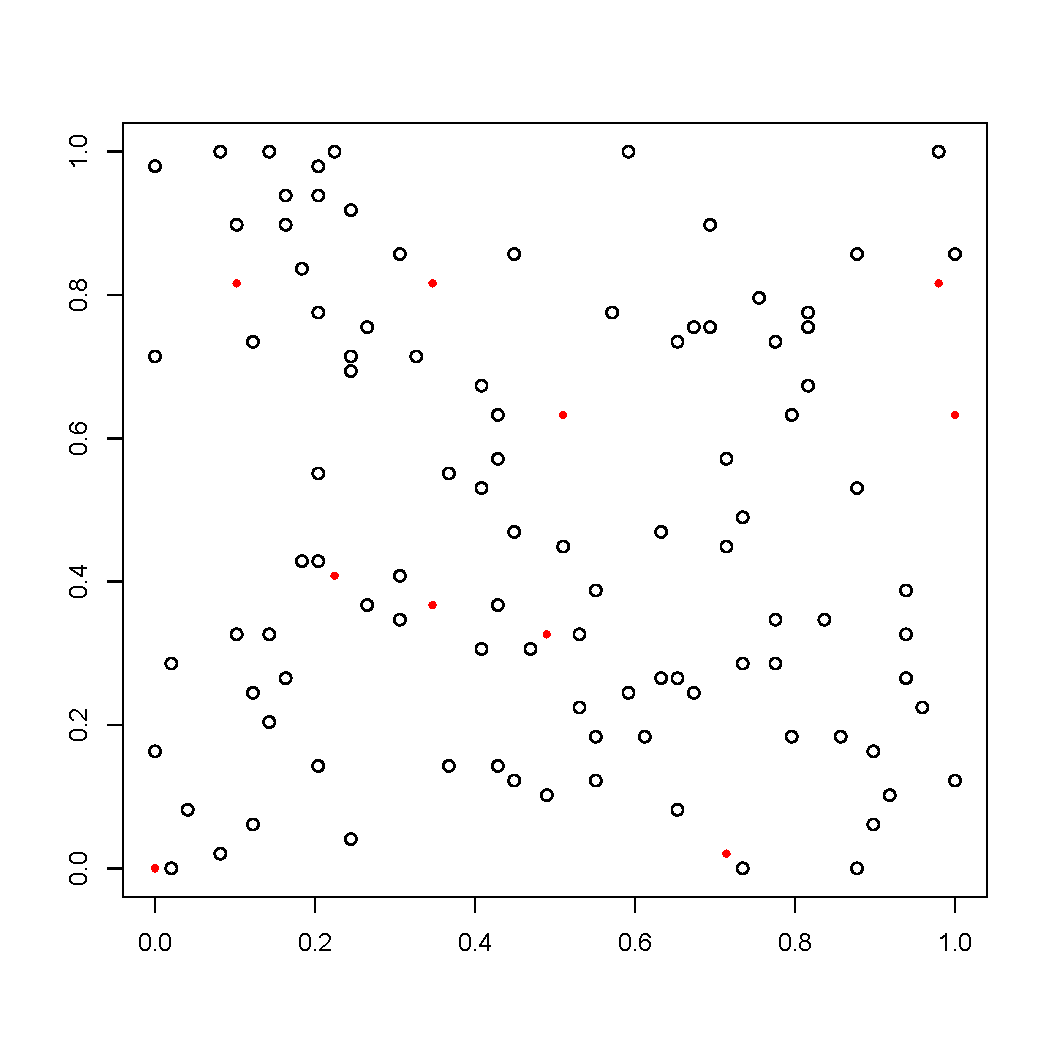
\includegraphics[width=0.5
		\textwidth]{images/kriging/locations.pdf} 
	\end{center}
	\caption{Locations of simulated curves. Solid dots are prediction locations.} \label{fig:locations} 
\end{figure}
\begin{figure}
	\begin{center}
		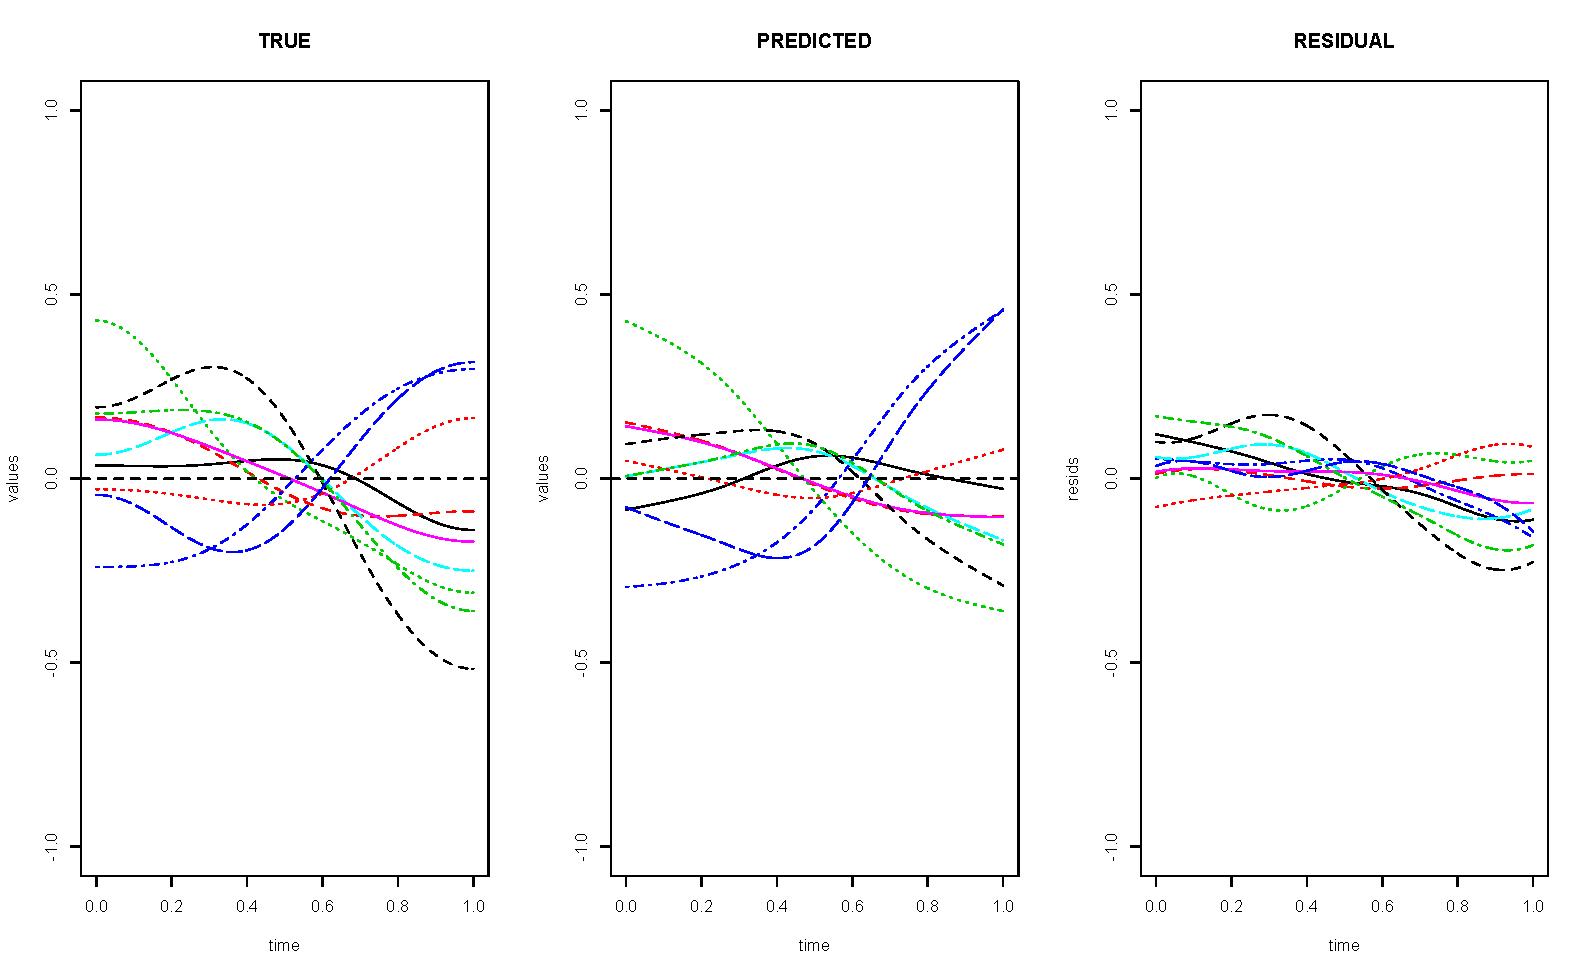
\includegraphics[width=0.6
		\textwidth]{images/kriging/residual-curves.pdf} 
	\end{center}
	\caption{Predicted curves at unobserved locations. } \label{fig:curve kriging predictions} 
\end{figure}

% section numerical_experiments (end)


\newpage

%===========================================
\section{Investigating the effects of spatial dependence} 

% (fold)
\label{sec:investigating_the_effects_of_spatial_dependence}

This section describes our effort toward gaining a better understanding of how the covariance function estimator, from which the principal component functions are derived, performs when the independence assumption is violated. We explores possible modifications to the covariance function estimator that account for spatial dependence. 

\subsection{Simulation framework useful for studying spatial dependence between curves} By using the simulation framework in Chapter \ref{ch:covariance estimation}, but using a spatially correlated Gaussian random variables instead of uniform random variables we can investigate the effects of spatial dependence on estimation of functional principal components. Already included here is a simulated example under independence. 

Random curves are simulated independently as 
\begin{equation}
	X(t) = \sum^{3}_{k=1}\zeta_k Z_k \cos(k\pi t), \hspace{0.5cm} t \in [0,1], \label{eq:sim process2} 
\end{equation}
where $Z_k$ were independently sampled from a $N(0,1)$ distribution and \(\zeta=(-1)^{k+1}k^{-\alpha}\). The covariance function for this process can be easily show to be 
\begin{equation}
	C(s,t) = \sum^{3}_{k=1}k^{-2\alpha} \cos(k\pi s)\cos(k\pi t). 
\end{equation}

Figure \ref{fig:sim curves2} shows 100 curves simulated independently from the process in \eqref{eq:sim process} with $\alpha=2$. 

% simulated curves
\begin{figure}
	\begin{center}
		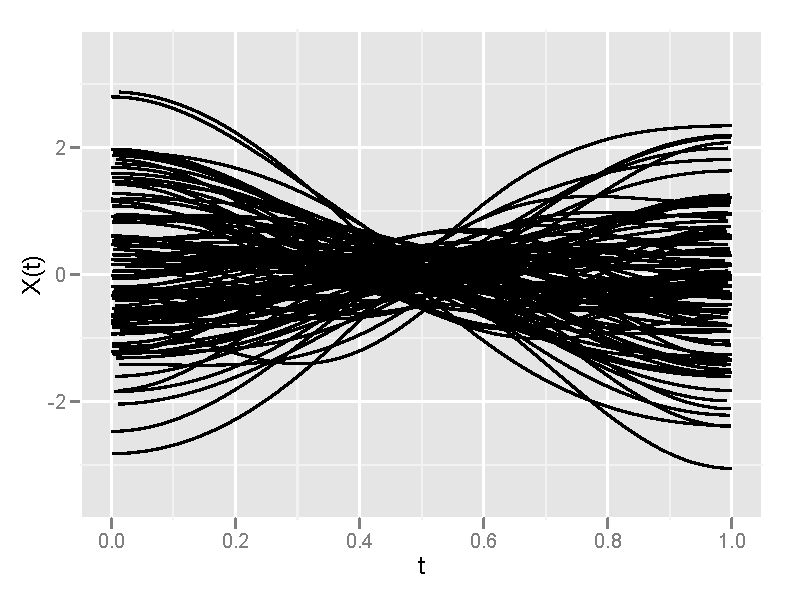
\includegraphics[width=0.5
		\textwidth]{images/Ch3/sim-curves.pdf} 
	\end{center}
	\caption{One hundred curves simulated independently from the process $X(t)$ in \eqref{eq:sim process2}.} \label{fig:sim curves2} 
\end{figure}

% estimated first FPC
\begin{figure}
	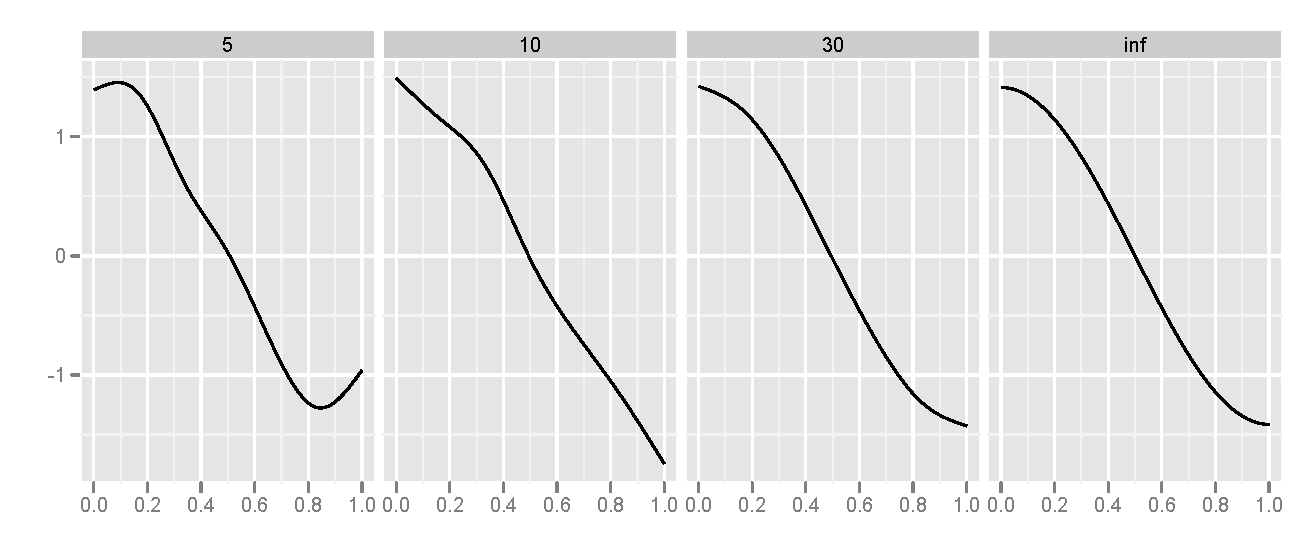
\includegraphics[width=
	\textwidth]{images/Ch3/eigenfun1-sig-0368.pdf} \caption{1st eigenfunction estimated from 100 simulated curves, where each curves is observed at $m$ random locations with noise ($\sigma = 0.0368$). The number of observations per curve is indicated in the plot label. } 
\end{figure}

% estimated second FPC
\begin{figure}
	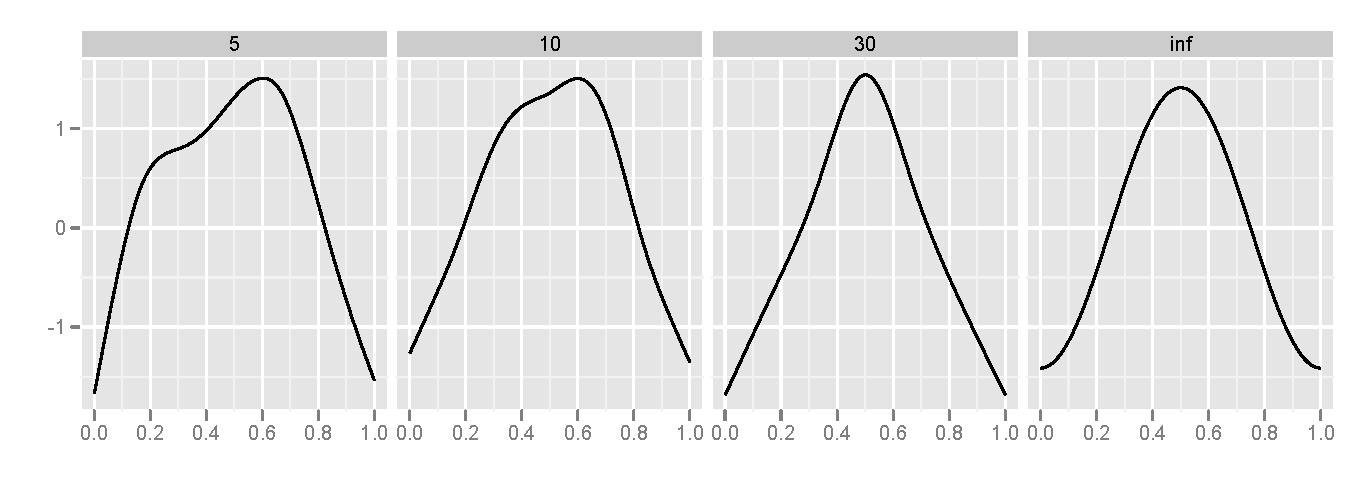
\includegraphics[width=
	\textwidth]{images/Ch3/eigenfun2-sig-0368.pdf} \caption{2nd eigenfunction estimated from 100 simulated curves, where each curves is observed at $m$ random locations with noise ($\sigma = 0.0368$). The number of observations per curve is indicated in the plot label. } 
\end{figure}

\newpage 
\subsection{Adjustments to the covariance function estimation which account for spatial dependence} \label{sec:adjustments to the covariance}

Let $\mathbf{b}^{(i)} = [(y_{ij}-\mu(t_{ij}))(y_{ij'}-\mu(t_{ij'}))]_{1\leq j\neq j'\leq m}$, $i=1, \dots, n$. Let
\[ \mathbf{b} = (\mathbf{b}^{(1)T}, \mathbf{b}^{(2)T}, \dots, \mathbf{b}^{(n)T} )^T, \]
then the vectors $\mathbf{b}^{(i)}$ contain values related to the sample covariance from curve $i$, and the vector $\mathbf{b}$ contains all sample covariance terms. The elements of $\mathbf{b}$ have non-trivial covariances due to spatial correlation among curves. However, we show that the elements of Cov$(\mathbf{b})$ can be compute using only covariances of the form \eqref{eq:cov}. Let
\[ \mathbf{W}= \text{Cov}(\mathbf{b}), \]

then elements of $\mathbf{W}$ can be computed as follows, 
\begin{align}
	\text{Cov}(\epsilon(s_i; t_{j}) \epsilon(s_i;t_{j'}), \epsilon(s_{i'}; t_{l}) \epsilon(s_{i'};t_{l'}) ) &= \text{Cov}(\epsilon(s_i; t_{j}), \epsilon(s_{i'}; t_{l}))\text{Cov}( \epsilon(s_i;t_{j'}), \epsilon(s_{i'};t_{l'}) ) \nonumber \\
	&+ \text{Cov}(\epsilon(s_i; t_{j}), \epsilon(s_{i'};t_{l'}) )\text{Cov}(\epsilon(s_i;t_{j'}), \epsilon(s_{i'}; t_{l})) \label{eq:cov of products} 
\end{align}
The right hand side of \eqref{eq:cov of products} holds under the assumption of Gaussian distributions (see \cite{Bohrnstedt:2010ud}). 

We propose the following estimator
\[ \widehat{C}_{\lambda}=\stackrel[C \in \H\otimes \H]{}{\text{ argmin}} \left\{ l_{n}(C)+\lambda\left\Vert C\right\Vert _{\breve{\H}}^{2} \right\}, \]
where 
\begin{equation}
	l_{n}(C)= (\mathbf{b} - \mathbf{C})^T\mathbf{W}^{-1}(\mathbf{b} - \mathbf{C}) \label{eq:weighted loss function} 
\end{equation}
and
\[ \mathbf{C} = [C(t_{i,j}, t_{i'j'})] \]

Though computation of $\mathbf{W}^{-1}$ is theoretically possible, the dimension of $\mathbf{W}$ is computationally prohibitive. 

We propose a computationally simpler way to adjust for spatial dependence using a weighting scheme motivated by the fundamental principle in spatial statistics, which states that data in close proximity contribute similar information; hence should be down weighted relative to data at sparse locations. Deriving a single weight for each curve corresponds to a diagonal $\mathbf{W}$ matrix in \eqref{eq:weighted loss function}. 

Define location intensity as the number of locations per unit area (a familiar concept in spatial point processes). In order to quantify the sentiment in the previous paragraph we propose estimating the intensity for each location, denoted by $\gamma_k$, and define a weight function 
\begin{equation}
	w_k = \left(\frac{1}{\gamma_k}\right)^p. 
\end{equation}

Let $\mathbf{W} = diag(\mathbf{w}_1, \dots, \mathbf{w}_n)$, then the covariance estimator is adjusted by defining the loss function as 
\begin{equation}
	l_{n}(C)= (\mathbf{b} - \mathbf{C})^T\mathbf{W}(\mathbf{b} - \mathbf{C}). \label{eq:diag weighted loss function} 
\end{equation}
We investigate the effect of adjusting for spatial dependence in this manner by simulating curves from a grid consisting of group of locations that are spars (low point intensity) and a clustered group of locations (high point intensity) shown in Figure~\ref{fig:grid3}. Different levels of spatial dependence are modeled through the value of the range parameter on a exponential covariance function,
\begin{equation}
	cov(s_j, s_k) = \sigma^2e^{-\frac{\norm{s_j - s_k}}{r}}. 
\end{equation}

Figure~\ref{fig:exp_corr_funs} shows the exponential correlation functions that correspond to the range values used ($r = 0.1, 0.2, 0.3$; $\sigma^2=1$). We used 20 observations per curve and a negligible noise variance. 

% plot of locations used to simulate curves
\begin{figure}
	\begin{center}
		\includegraphics[width=
		\textwidth]{Images/kriging/grid3.pdf} 
	\end{center}
	\caption{Locations of curves used for the simulation.} \label{fig:grid3} 
\end{figure}

% plot of exponential covariance functions
\begin{figure}
	\begin{center}
		\includegraphics[width=
		\textwidth]{Images/kriging/exp_corr_funs.pdf} 
	\end{center}
	\caption{Exponential covariance functions used in the simulation.} \label{fig:exp_corr_funs} 
\end{figure}

% plots of MSE vs spatial weight values for different values of spatial dependence
\begin{figure}
	\begin{center}
		\includegraphics[width=
		\textwidth]{Images/kriging/MSE_trends.pdf} 
	\end{center}
	\caption{The x-axis shows the value of the scale parameter, $p$, in the weight function. Large values of p correspond to smaller weights for curves in high point intensity areas. The y-axis shows the average integrated square error for the covariance estimator. The error bars show +/- standard error for the mean, and the size of the dots corresponds to the sample size for each mean (ultimately these should be equal, but currently they are not). The dotted line show values for independent curves.} \label{fig:MSE_trends} 
\end{figure}
% sec:investigating_the_effects_of_spatial_dependence (end)

\section{Discussion} % (fold)
\label{sec:discussion}
Put discussion here
% section discussion (end)

%\todo[inline]{discuss how possible measures of interest (e.g. min, max, average) are functionals of the curve predictor. Should this go in the introduction? }
